\chapter{Diseño y modelado}

\section{Arquitectura}
ALTEM es una aplicación web de Stack Completo la cual está compuesta por las siguientes tecnologías
\begin{itemize}
    \item Front-End: Javascript ES5 con AngularJS 1.6
    \item BackE-End: PHP 7.1 con Laravel.
    \item Bases de Datos: SQL por MySQL.
\end{itemize}

Su API también se comunica con otros sistemas que pertenecen a la universidad, tales como

\begin{itemize}
    \item LDAP (Actualmente Deprecado)
    \item SAVIO (Moodle)
    \item Banner (Oracle)
\end{itemize}

En la Figura 3.1 Se puede apreciar la Arquitectura de ALTEM y la relacion existente entre cada uno de los elementos del stack y las APIs externas. 

\begin{figure}[H]
    \centering
    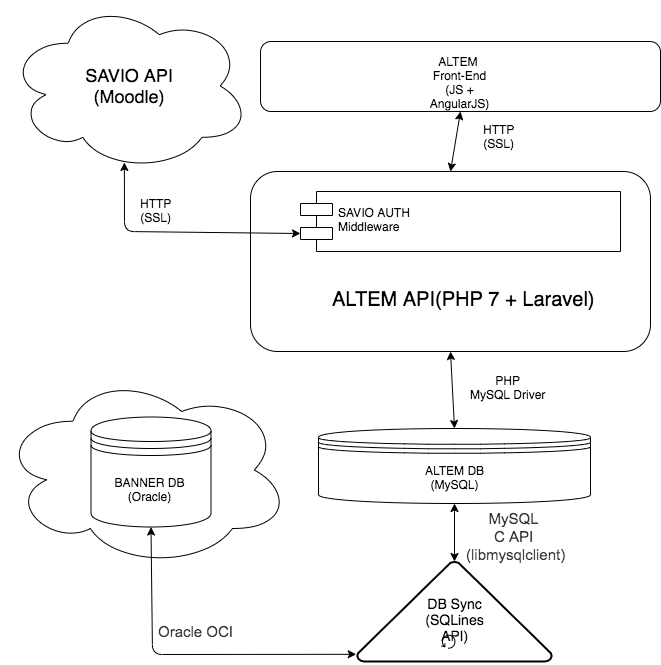
\includegraphics[width=0.7\textwidth]{img/ALTEM.png}
    \caption{Arquitectura de ALTEM}
\end{figure}

\subsection{Cliente (Front-End)}
Al ser una aplicacion web, ALTEM se consume desde el navegador, por medio de un Front-End creado en HTML5, CSS y JavaScript.

La capa de JavaScript está manejada por AngularJS 1.6, el cual nos facilita el desarrollo de las funcionalidades utilizando el patrón MVC el cual es un patrón de arquitectura de software, que separa los datos y la lógica de negocio de una aplicación de su representación, y el módulo encargado de gestionar los eventos y las comunicaciones.
MVC propone la construcción de tres componentes distintos que son el modelo, la vista y el controlador, es decir, por un lado define componentes para la representación de la información, y por otro lado para la interacción del usuario.\cite{trygve}

La aplicación web está compuesta por varios módulos, cada uno con sus modelos, vistas y controladores.

Los módulos son los siguientes:

\begin{itemize}
    \item Acción
    \item Estrategia
    \item Filtros
    \item Login
    \item Reportes
    \item Riesgos
    \item Tipos de Riesgos
    \item Usuarios
\end{itemize}

\subsubsection{Modelo}
Para el caso del cliente web, nuestro modelo equivale a todos los datos que vienen desde la API y que se solicitan por medio de peticiones HTTP. Estos datos se guardan en el localStorage y sessionStorage, y representan toda la información que el usuario puede ver a través de la vista en tiempo real.

Estas solicitudes a la API se encuentran organizadas en Servicios\cite{servicios} los cuales ejecutan llamadas a distintos endpoints\cite{endpoints}.

\begin{itemize}
    \item Acción
    \item Archivo Personal
    \item Criterio
    \item Estrategia
    \item Estudiante
    \item Filtro
    \item Intervención
    \item Login
    \item Observación
    \item Reporte
    \item Riesgo
    \item Tipo Riesgo
    \item Usuario
\end{itemize}

Estos servicios se comunican con el Back-End a trvés de la API de XMLHttpRequest(XHR) y utilizando métodos HTTP.

El Modelo es modificado por los Controladores, los cuales actualizan el estado de los datos dependiendo de las interacciones que tenga la aplicación con el usuario.
\subsubsection{Controlador}
Los controladores son funciones que disparan las instrucciones que modifican el Modelo, generalmente llamadas en la vista a través de eventos y en los servicios a través de Promesas.
En la aplicación web, todas las acciones (iniciar sesión, ver estudiantes, añadir estrategias, filtrar búsquedas, etc) disparan estos controladores, estos controladores se encuentran categorizados por los módulos mencionados en 1.1.

Las funciones principales de los controladores en la aplicación web son los siguientes:

\begin{itemize}
    \item Mutar el estado local de la aplicación.
    \item Hacer llamadas a los servicios.
    \item Actualizar la Vista.
\end{itemize}

Por lo general, las acciones ejecutadas en los controladores hacen que la vista se refresque.

\subsubsection{Vista}
La Vista se concibe como la capa presentacional de la aplicación web. Es la parte que interactúa con el usuario directamente y es la que se encarga de renderizar todos los datos del modelo en una manera que el usuario puede comprender fácilmente. 

Las vistas están hechas a través de plantillas HTML5 estilizadas con CSS, las cuales se renderizan de forma dinámica a medida que el modelo de la aplicación se actualice y se vayan ejecutando eventos que disparen los controladores.

La vista también se actualiza por medio de las directivas de AngularJS.

\subsection{Servidor (Back-End)}
El Back-End es el núcleo de ALTEM, consiste en una app Laravel y PHP7 en la que se encuentra toda la lógica del servidor.
Al igual que el Front-End, esta aplicación comparte la misma arquitectura MVC, pero orientada al lado del servidor.

También, se encarga de comunicarse con API's de terceros como BANNER y SAVIO, plataformas pertenecientes a los recursos tecnológicos de la Universidad Tecnológica de Bolívar para obtener datos esenciales para su funcionamiento, de los cuales hablaremos más adelante. 

\subsubsection{Modelo}
Para nuestro Back-End, el Modelo es una representación de la estructura de los datos y relaciones que se manejan  base de datos, en clases y objetos que comparten la misma estructura. Esto con el propósito de que se maneje una consistencia entre la base de datos y la API.

Para hacer esa integración posible, se utiliza una API llamada Eloquent, la cual nos permite construir y ejecutar consultas a la base de datos utilizando definiciones y métodos propios del lenguaje. Esto también se conoce como ORM.

Para cada tabla existente en la base de datos, existe un modelo correspondiente en el back-end el cual se representa mediante una Clase como lo muestra el siguiente ejemplo:

\begin{lstlisting}
namespace App\Models;

class Tabla extends Model
{
    protected $table = 'nombre_tabla';
    
    // columnas de la tabla
    protected $fillable = ['columna1', 'columna2', 'columna3'];

    //PK
    protected $primaryKey= "codigo";

    // Relaciones
    public function relacion1()
    {
        // Ejemplo 1:N
        return $this->belongsToMany('OtroModelo','FK','FK','FK');
    }

    public function relacion2(){
        // Ejemplo 1:1
        return $this->hasOne('OtroModelo','FK','FK');
    }
}
\end{lstlisting}

Esta clase extiende de Model, la cual es una clase implementada por Laravel para manejar las relaciones entre tablas. Esa clase posee varios metodos como los observados previamente.

\subsubsection{Controlador}
En el caso del Back-End, los controladores son clases que poseen los métodos que ejecutan la lógica de la aplicación y hacen los cambios en la base de datos al llamar a los Modelos

Una clase controladora se compone de la siguiente manera:

\begin{lstlisting}
namespace App\Http\Controllers;

// importamos Modelo relacionado con el controlador
use \Models\Tabla;

class Acciones extends Controller
{
    public function __construct()
    {
        // Usamos middlewares necesarios
        $this->middleware('cors');
    }

    public function obtener_todos()
    {
       $datos = Tabla::all();
        return response()->json($datos);
    }
    
     public function obtener_por_codigo($codigo)
    {
        $datos_codigo = Tabla::find($codigo);
        return response()->json($datos_codigo);
    }
    
      public function eliminar_por_codigo($id)
    {
        $datos_de_id = Tabla::find($id);
        $datos_de_id->delete();
        return response()->json(["mensaje" => "Eliminado con Exito"]);
    }
}
\end{lstlisting}

En este ejemplo, podemos observar como la la clase Acciones posee varios métodos que llaman a Modelo y ejecutan varios métodos sobre este. Estos métodos representan consultas SQL que modifican los datos en la base de datos.
Al final de las instrucciones, se retornan los datos solicitados o el mensaje por medio de JSON.

\subsubsection{Vista}
Al ser una API, en este caso la vista no representa ninguna capa de interacción con el usuario sino más bien un conjunto de rutas o endpoints los cuales son consultados mediante HTTP y que son el puente entre el Back-End y el Front-End.

\subsection{Bases de Datos}
ALTEM se alimenta de 2 bases de datos \textbf{ALTEM} y \textbf{SIRIUS}

Las bases de datos de ALTEM son de tipo SQL, ejecutadas en el motor MySQL X, todas las consultas son manejadas por el ORM del Back-End

\subsubsection{ALTEM DB}
En esta base de datos se guarda toda la información relacionada a los procedimientos que se le hacen a los estudiantes que se encuentren en una situación de riesgo.
Al ser una base de datos Relacional, fue necesario establecer un conjunto de relaciones entre tablas para mantener la consistencia y confiabilidad en los datos utilizados en la aplicación, como se aprecia en la Figura 3.2.

\begin{figure}[H]
    \centering
    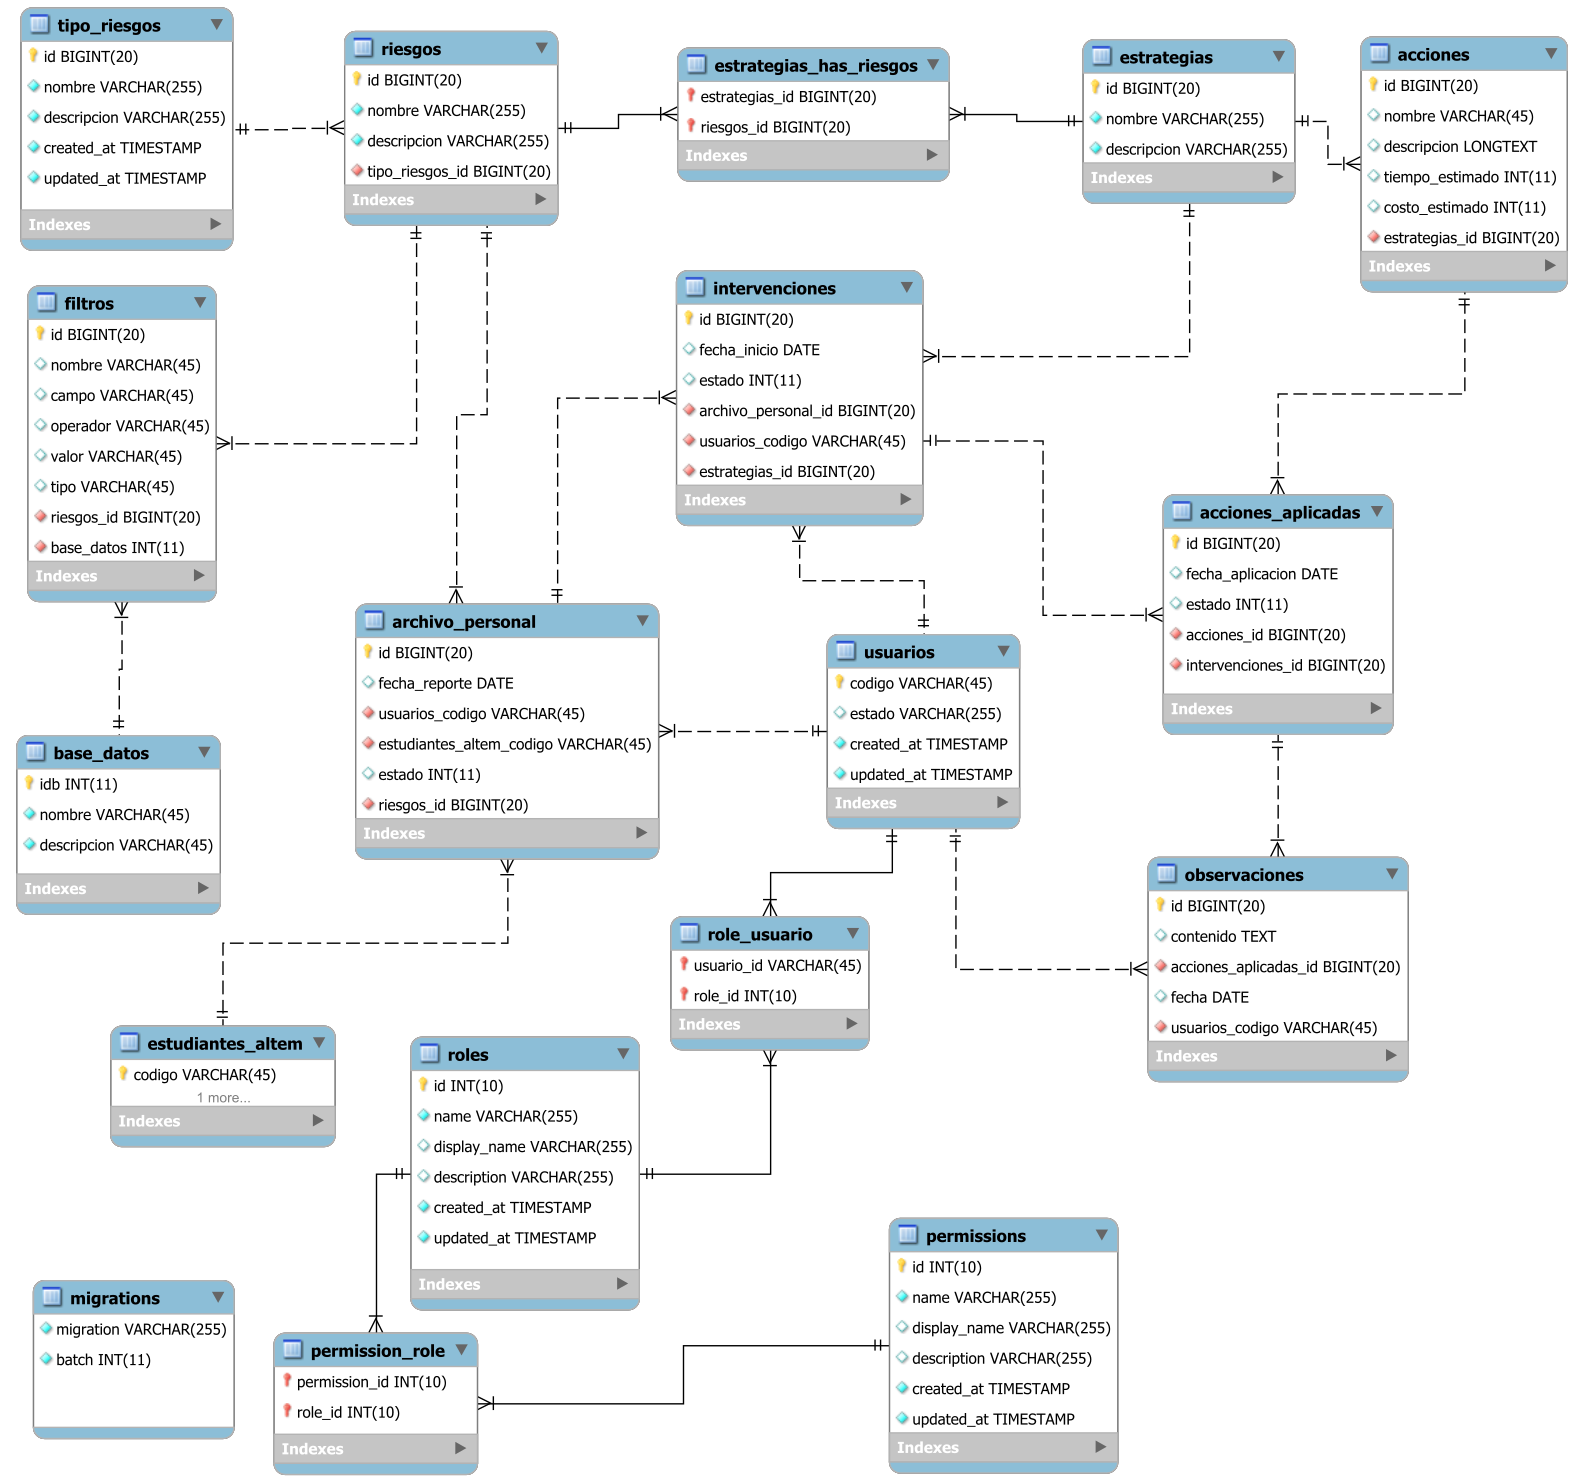
\includegraphics[width=1\textwidth]{img/EER.png}
    \caption{Relación de entidades en la base de datos de ALTEM.}
\end{figure}

\subsubsection{SIRIUS DB}
SIRIUS es una base de datos que se creó como una copia de los registros estudiantiles en SIRIUS (Ahora BANNER), esta base de datos se sincronizaba por medio de un script que leía los datos en SIRIUS e importaba todo hacia esta base de datos.

Actualmente, SIRIUS evolucionó a BANNER y algunas tablas cambiaron, como por ejemplo la tabla de ESTUDIANTEs y DATOS\_ACADEMICOS, en las que cambió la collation, el tamaño de los datos de algunas columas y los nombres de algunas columnas también.

\section{Plan de trabajo}
\subsection{Reunión con Consejeros}
Se realizó una reunión con los consejeros de bienestar universitario y se concluyó en que ALTEM debía ser intervenido para que su funcionamiento volviese a la normalidad, y se plantearon un conjunto de mejoras las cuales pasaron a ser nuevos requerimientos para la aplicación.

De acuerdo a los análisis realizados en ALTEM para determinar su estado funcional y de implementación, se concluyó que la aplicación podría mejorarse si se cumplen estos nuevos requerimientos y se solucionan las fallas que impiden su funcionamiento.

\subsection{Identificación de las Fallas Críticas}
Se realizó una revisión de ALTEM en el entorno de producción, el cuál se encontraba en estado de abandono y desuso por parte de los consejeros debido a que manifestaron que el sistema se había vuelto imposible de usar debido a fallas en su funcionamiento. 
En esta revisión inicial se identificaron las principales fallas: 

\begin{itemize}
    \item No se podía acceder a la plataforma debido a problemas con la autenticación.
    \item No se podían crear nuevos registros debido a que el servidor no tenía almacenamiento.
    \item No se podía obtener información estudiantil debido a que no había conexión con SIRIUS (Ahora BANNER).
\end{itemize}

Estas fallas hicieron que la aplicación dejara de funcionar en su totalidad, ya que afectaron componentes esenciales de su arquitectura.

\subsection{Definición de Requerimientos}
Luego de analizar las peticiones de los consejeros y de encontrar todas las fallas en la aplicación, se desarrollaron los siguientes requerimientos:

\begin{itemize}
    \item Conectar, consumir y sincronizar los datos académicos y estudiantiles de ALTEM con el nuevo sistema BANNER.
    \item Hacer mejoras en las interfaz de usuario ya que no es posible determinar cuando un elemento está cargando.
    \item Analizar las falencias en la experiencia de usuario y hacer mejoras en ese aspecto.
    \item Resolver las fallas (bugs) presentes en la aplicación.
    \item Hacer refactorización de los módulos que presentan problemas de calidad de código y arquitectura.
    \item Implementar los nuevos requerimientos solicitados el personal de consejería académica
\end{itemize}

\subsection{Plan de Desarrollo}
Se decidió implementar la metodología Ágil SCRUM como estrategia para llevar a cabo el plan de trabajo.

Se agruparon todas requisitos en Epics, Historias de usuario, y Tareas.

\subsubsection{Epics}
Todas las tareas e Historias de Usuario se agruparon en dos Epics principales, los cuales se diferencian por prioridad, ya que fue necesario resolver las tareas e historias de usuario de un Epic primero para poder empezar con el siguiente.
Los Epics creados fueron los siguientes

\subsubsection{Historias de Usuario}
(aqui hablo acerca de como cree cada historia de usuario y de que hice en cada unia)

Luego de analizar los requerimientos y las recomendaciones planteadas por los consejeros se desarrollaron las siguientes historias de usuario las cuales representan las nuevas funcionalidades a implementar:

\begin{itemize}
    \item Como consejero debo poder iniciar sesión en ALTEM con mis credenciales de SAVIO.
    \item Como consejero debo poder ver los datos estudiantiles que me provee BANNER.
    \item Como consejero debo poder descargar un reporte de mis casos activos en MS EXCEL.
    \item Como consejero deseo ver el periodo en el que se presentó algún tipo de riesgo en el estudiante.
    \item Como consejero deseo poder añadir anotaciones a los estudiantes.
    \item Como administrador deseo gestionar qué cuáles usuarios de SAVIO pueden acceder a la aplicación.
\end{itemize}

\subsubsection{Errores de la aplicación}

\begin{itemize}
    \item Para algunos estudiantes no es posible finalizar una acción.
    \item No se está mostrando la información de los estudiantes actualizada.
    \item 
\end{itemize}

\subsubsection{Plan de desarrollo}


(aqui hablo de como desarrollé mi plan de trabajo de acuerdo a una metodología agil)

\subsubsection{creacion de bugs/requerimientos}
(aqui hablo acerca de como encontré cada bug y resolvi cada issue )

\subsection{QA}
(aqui hablo de como probé la fuincionalidad, como fueron las pruebas unitarias y todo eso)
